\chapter{\IfLanguageName{dutch}{Stand van zaken}{State of the art}}
\label{ch:stand-van-zaken}

% Tip: Begin elk hoofdstuk met een paragraaf inleiding die beschrijft hoe
% dit hoofdstuk past binnen het geheel van de bachelorproef. Geef in het
% bijzonder aan wat de link is met het vorige en volgende hoofdstuk.

% Pas na deze inleidende paragraaf komt de eerste sectiehoofding.

In deze studie lees je alles over het OAuth-framework en wat de rol van azure hierin is. Het doel van deze studie is om een nauwgezet beeld te krijgen van het onderwerp om zo op de hoogte te zijn van de huidige stand van zaken in het onderzoeksdomein. Deze studie focust zich op volgende vragen. Wat houdt het OAuth-framework in? Waarom was er vraag naar een nieuw authorization framework? Wat heeft azure active directory hiermee te maken? Ook zal duidelijk het verschil tussen authorization en authenticatie uitgelegd worden om daarna kort in te gaan op openID, een framework dat bovenop OAuth geplaatst kan worden.
\section{\IfLanguageName{dutch}{Het OAuth-framework}{The OAuth-framework}}
\label{sec:OAuthFramework}
Om de onderzoeksvraag correct te beantwoorden is het belangrijk dat er eerst diep wordt ingegaan op het doel en de flow van het authorization framework OAuth.

OAuth is een framework dat het mogelijk maakt voor gebruikers om applicaties toegang te geven tot hun gegevens in applicatie van derden zonder hier hun wachtwoord voor te moeten geven \autocite{Deniss2016}.

Voor het begrijpen van OAuth is het belangrijk dat enkele termen geassocieerd worden met hun juiste betekenis. Het OAuth-framework heeft drie onderdelen die essentieel zijn om de flow goed te begrijpen. Hier wordt gesproken over een client, een api en een user, zoals afgebeeld in figuur \ref{fig:oauth1} \autocite{Services2016}.
\begin{figure}[H]
	\centering
	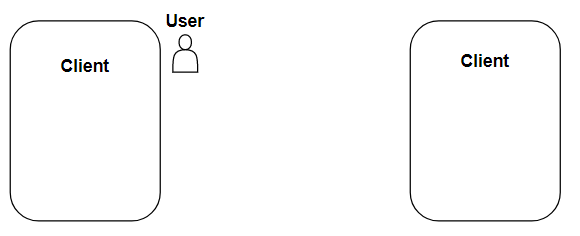
\includegraphics{OAuthFlow1} 
	\caption[Visueel de drie componenten]{Hier zijn visueel de drie componenten van OAuth afgebeeld.}
	\label{fig:oauth1}
\end{figure}
De flow kan uitgelegd worden aan de hand van een voorbeeld. In dit voorbeeld wordt als client een webapplicatie genomen. De api wordt dan voorgesteld als de authorization en resource server van de applicatie waar de webapplicatie de gebruikergegevens van wenst. Om het gemakkelijk te houden zal dit hier Facebook zijn. Merk wel op dat de authorization server niks van persoonlijke informatie over de gebruiker heeft, deze is puur voor authorization. De persoonlijke gegevens en resources van de gebruiker zijn allemaal te vinden op de resource server. Voor de user wordt de naam Jan gebruikt. Dit voorbeeld wordt visueel afgebeeld op figuur \ref{fig:oauth2} \autocite{Deniss2016} \autocite{Services2016}.
\begin{figure}[H]
	\centering
	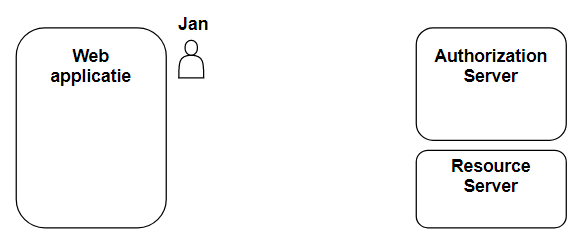
\includegraphics{OAuthFlow2} 
	\caption[De drie componenten aan de hand van een voorbeeld]{Hier zijn visueel de drie componenten van OAuth afgebeeld aan de hand van een voorbeeld.}
	\label{fig:oauth2}
\end{figure}
In dit voorbeeld wenst de gebruiker Jan zijn contacten van Facebook te synchroniseren met zijn contacten op de webapplicatie. Hiervoor heeft de webapplicatie dus de gegevens van Jan nodig die op de resource server van Facebook staan, maar dit zonder het wachtwoord van Jan te weten. Hoe gaat dit in zijn werk?
De eerste stap is dat Jan vraagt om zijn contacten te sychroniseren door op een knop op de webapplicatie te klikken. Wanneer hierop geklikt wordt begint OAuth met het uitvoeren van de flow. De webapplicatie zal een aanvraag sturen naar de authorization server van Facebook en de server zal een inlog scherm tonen aan de gebruiker. Jan kan nu inloggen met zijn gegevens van Facebook op de authorization server. Dit zie je visueel op figuur \ref{fig:oauth3} \autocite{Services2016} \autocite{OktaDev2018}.
\begin{figure}[H]
	\centering
	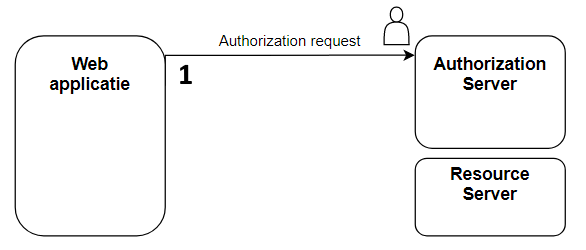
\includegraphics{OAuthFlow3} 
	\caption[Eerste call naar de authorization server]{Hier wordt visueel de eerste call naar de authorization server afgebeeld.}
	\label{fig:oauth3}
\end{figure}
Wanneer Jan heeft ingelogd op de authorization server en een eventueel extra toestemmingsscherm aanvaard heeft, zal de server een authorization grant, waar zich een authorization code in bevindt, terugsturen naar de webapplicatie. Dit is afgebeeld op figuur \ref{fig:oauth4}  \autocite{Services2016}.
\begin{figure}[H]
	\centering
	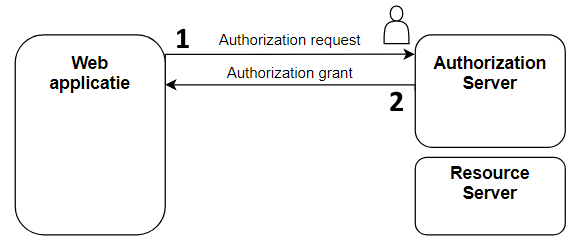
\includegraphics{OAuthFlow4} 
	\caption[Authorization grant wordt teruggestuurd]{Hier wordt visueel afgbeeld dat de authorization server een authorization grant terugstuurd naar de webapplicatie.}
	\label{fig:oauth4}
\end{figure}
De webapplicatie gaat nu deze authorization grant die de authorization code bevat naar de authorization server sturen om zo aan een access token te komen. Deze access token is in de vorm van een bearer token. Deze token zal later gebruikt worden om aan de gegevens van Jan op de resource server te kunnen. Wanneer de authorization server de authorization grant en code van Jan goedkeurt zal deze een access token terugsturen naar de webapplicatie (figuur \ref{fig:oauth5})  \autocite{Services2016} \autocite{OktaDev2018}.
\begin{figure}[H]
	\centering
	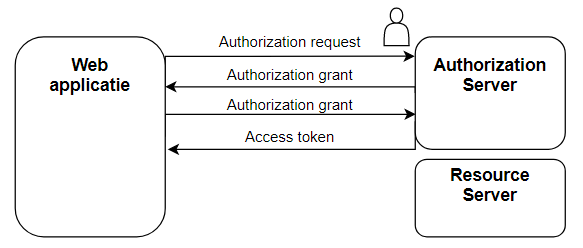
\includegraphics{OAuthFlow5} 
	\caption[Ophalen van de access code]{Hier wordt afgebeeld hoe de webapplicatie die authorization grant terugstuurt naar de authorization server om zo een access code te bemachtigen.}
	\label{fig:oauth5}
\end{figure}
Nu er een geldige access token bemachtigd is, heeft de webapplicatie toegang tot de resource server om zo aan de gegevens van Jan te kunnen. Natuurlijk is het niet de bedoeling dat de webapplicatie zomaar aan alle gegevens van Jan kan. Om dit te vermijden is er nog een belangrijke term binnen OAuth, namelijk scopes. Een authorization request is altijd scoped. Dit betekent in dit voorbeeld dat de authorization request scoped was om enkel de contacten van Jan te bekijken. De webapplicatie kan dus enkel de contacten raadplegen en geen andere persoonlijke informatie van Jan \autocite{Services2016} \autocite{OktaDev2018}. 

Om nu dus aan de contacten van Jan te komen, gaat de webapplicatie dit verzoek naar de resource server sturen met de access token inbegrepen. De resource sever gaat dan kijken of de access token correct is en zo de contacten gaan ophalen en terugsturen naar de webapplicatie (figuur \ref{fig:oauth6}) \autocite{Services2016} \autocite{OktaDev2018}.

\begin{figure}[H]
	\centering
	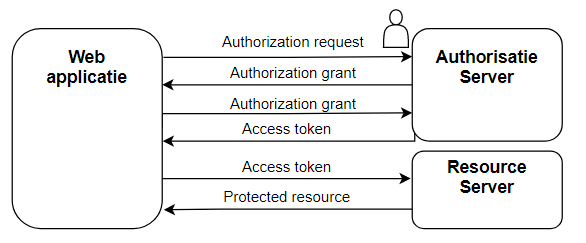
\includegraphics{OAuthFlow6} 
	\caption[Gebruik van access token voor ophalen protected resource]{Hier wordt afgebeeld hoe de webapplicatie met de access token de protected resources van de user gaat ophalen.}
	\label{fig:oauth6}
\end{figure}
Merk op dat OAuth hier dient als het authorization framework. De authentication van de gebruiker Jan gebeurt met openId connect door het gebruik van id-tokens die mee gegeven worden met de access token \autocite{OktaDev2018}.

Om dit allemaal te laten werken is er een belangrijke stap die niet vergeten mag worden. Voordat de webapplicatie deze flow kan hanteren met een api, in dit geval Facebook, moet de webapplicatie zich eerst registreren bij de Facbook api service. Om dit te doen moet de webapplicatie zijn naam, website en callback url opgeven. Een callback url is simpelweg een url naar waar de api zal redirecten na het identificeren van de gebruiker. Wanneer de webapplicatie deze gegevens aan de api service gegeven heeft, krijgt deze een clientId en een client secret terug. Een cleintId is een publieke en unieke key die gebruikt wordt om de webapplicatie te identificeren als applicatie. De client secret is een private key die geheimgehouden wordt tussen de applicatie en de api. Deze secret wordt gebruikt om de applicatie te identificeren wanneer deze een verzoek doet voor een access token \autocite{OktaDev2018}. 

\subsection{\IfLanguageName{dutch}{Grant types van OAuth}{Grant types of OAuth}}
Om de vier verschillende grant types van OAuth te bekijken is het belangrijk bovenstaand voorbeeld meer in detail te bekijken (figuur \ref{fig:grantTypes1}).
\begin{figure}[H]
	\centering
	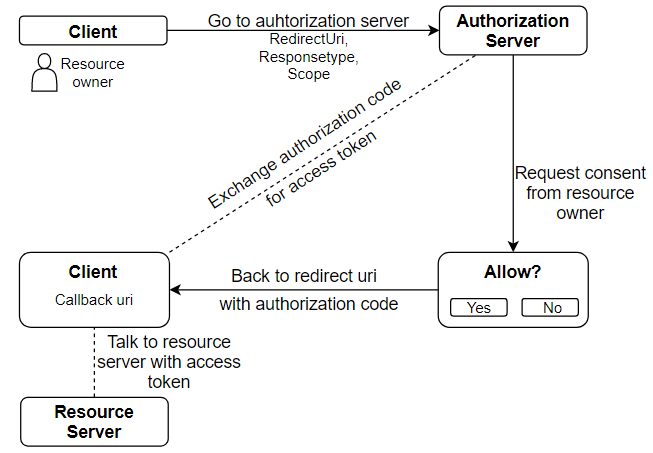
\includegraphics{GrantTypes1} 
	\caption[Gedetailleerd voorbeeld voor uitleg grant types]{Dit is het voorgaande voorbeeld gedetailleerd uitgewerkt.}
	\label{fig:grantTypes1}
\end{figure}
In deze figuur is dezelfde flow als het vorige voorbeeld uitgetekend. Het is belangrijk dit zo uit te tekenen voordat er verder wordt ingegaan op grant types.
Het eerste wat besproken moet worden is netwerkcommunicatie. Binnen netwerkcommunicatie zijn er twee mogelijke channels die gebruikt kunnen worden voor communicatie. Deze worden opgesplits in \autocite{OktaDev2018}: 
\begin{itemize}
	\item Back channel (highly secured)
	\item Front channel (less secured channel)
\end{itemize}
\subsubsection{\IfLanguageName{dutch}{Back channel (highly secured)}{Back channel (highly secured)}}
Een back channel is de veiligste channel van de twee om gegevens uit te wisselen. Deze uitwisseling gebeurt vaak over https, is vaak SSL encrypted en kan niet onderschept worden. Deze channel wordt vaak gebruikt voor communicatie tussen twee servers of api's \autocite{OktaDev2018}.
\subsubsection{\IfLanguageName{dutch}{Front channel (less secured channel)}{Front channel (less secured channel)}}
Front channel is minder beveiligd dan een back channel. Een goed voorbeeld van front channel communicatie is bijvoorbeeld de browser. Deze is veilig, maar als er gekeken wordt naar hoe een browser gebouwd is, valt op dat er loopholes of datalekken kunnen zijn. Alles wat met front channel verstuurd wordt, kan mogelijks zelfs gewoon in de url afgelezen worden \autocite{OktaDev2018}.
\subsubsection{\IfLanguageName{dutch}{Grant types}{Grant types}}
Bij het bekijken van figuur \ref{fig:grantTypes1} kan je een verschil zien tussen stippellijnen en volle lijnen. Deze staan voor welke channel er gebruikt wordt. Aangezien front channel minder beveiligd is dan back channel wordt deze gebruikt voor alles wat niet super beveiligd moet worden, zoals het uitwisselen van de authorization grant. Als dit onderschept zou worden, zou het niet zo erg zijn, met een authorization grant is een potentiele hacker niks \autocite{OktaDev2018}. 

Wat wel beveiligd moet worden, is de access token en mogelijke id-token. Als deze onderschept wordt door een potentiele hacker, kan deze aan de persoonlijke gegevens van de gebruiker op de resource server. Daarom wordt hiervoor de back channel gebruikt. Dit is ook meteen de reden waarom er tweemaal terug wordt gegaan naar de authorization server in plaats van dat deze in één keer de access token meestuurt in de front channel \autocite{OktaDev2018}.

Nu de verschillende channels zijn uitgeklaard kunnen de vier grant types van OAuth besproken worden. De vier grant types van OAuth zijn de volgende \autocite{OktaDev2018}:
\begin{itemize}
	\item Authorization code grant (front + back channel)
	\item Implicit (alleen front channel)
	\item Resource owner password credentials (alleen back channel)
	\item Client credentials (alleen back channel)
\end{itemize}
In \ref{fig:grantTypes1} zie je een voorbeeld van authorization code grant. Dit is de grant type die het meest gebruikt wordt bij webapplicaties met een server backend. Deze grant type is ook meteen de veiligste aangezien deze gebruik maakt van zowel front- als back channelcommunicatie \autocite{OktaDev2018}.

De op een na meest gebruikte grant type is implicit flow. Deze grant type is iets minder veilig dan authorization code grant, maar wordt vaak gebruikt bij bijvoorbeeld javascript applicaties \autocite{OktaDev2018}. 

Aangezien authorization code grant en implicit flow de meest gebruikte zijn zie je in figuur \ref{fig:grantTypes2} ook een visueel voorbeeld van een implicit flow. Nu is het mogelijk om duidelijk het verschil te zien in de flow.
\begin{figure}[H]
	\centering
	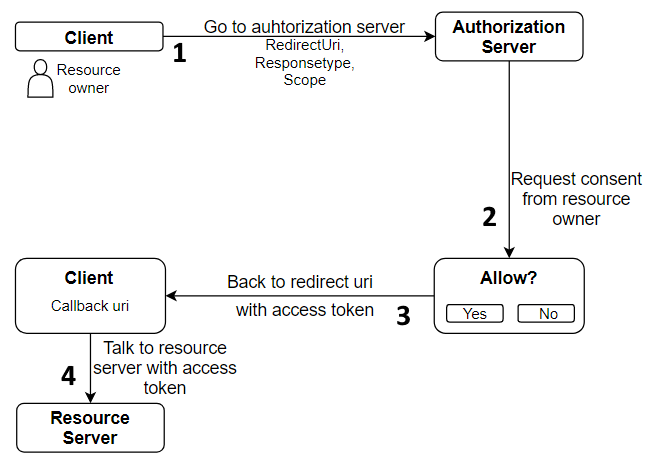
\includegraphics{GrantTypes2} 
	\caption[Visuele voorstelling van implicit grant]{Hier zie je het zelfde schema als de vorige voorbeelden, maar dan met implicit grant in plaats van authorization code grant.}
	\label{fig:grantTypes2}
\end{figure}
Zoals je kan zien in figuur \ref{fig:grantTypes2} zijn nu alle requests met volle lijnen in plaats van met stippellijnen. Dit komt dus omdat er bij implicit flow geen back channel communicatie gebruikt wordt. Hier gebeurt alles met front channel communicatie. Wat ook opvalt is dat hier meteen de access token door de authorization server wordt meegestuurd in plaats van eerst een authorization grant met authorization code. Er moest dus één request minder naar de authorization server gedaan worden. Het nadeel van deze flow is dus wel dat het minder veilig is dan authorization code grant \autocite{OktaDev2018}. 

Bij authorization code grant worden het uitwisselen van access token met de authorization server en alle communicatie met de resource server dus via de back channel gedaan. Dit is dus omdat deze access token niet in de verkeerde handen mag vallen. Bij elk request naar de resource server wordt deze access token ook mee gestuurd en daarom gebeuren deze requests ook via de back channel \autocite{OktaDev2018}.

De client credentials flow en resource owner password credentials worden minder gebruikt. Client credentials flow wordt soms nog gebruikt bij machine-naar-machinecommunicatie en resource owner password credentials wordt soms nog gebruikt om oudere applicaties juist te doen werken. Beide zijn ze echter niet meer aan te raden om te gebruiken \autocite{OktaDev2018}.

\subsection{\IfLanguageName{dutch}{Authentication vs authorization}{Authentication vs authorization}}
Zoals eerder vermeld is het OAuth-framework enkel bedoeld voor authorization, maar met enkele aanpassingen kan het ook gebruikt worden voor authentication. Maar wat is nu precies het verschil \autocite{rwike772020}?

Authentication is het proces van bewijzen dat je bent wie je zegt dat je bent. Dit is dus niet te vergelijken met authorization, dat dient om een geïdentificeerde partij toestemming te geven om iets te doen en om te bepalen tot welke gegevens deze partij toegang heeft \autocite{rwike772020}.

\subsection{\IfLanguageName{dutch}{OpenId connect}{OpenId connect}}
Als OAuth enkel bedoeld is voor authorization, wat is die id-token dan en hoe doe je aan authentication? Zoals gezegd kan je met een kleine aanpassing zorgen dat je met OAuth ook aan authentication kan doen. Dit framework heet openId connect. \autocite{rwike772019} \autocite{rwike772019a}

Toen openId connect nog niet bestond werd OAuth ook al door velen gebruikt, maar niet zoals het hoorde. Veel mensen vonden de authorization mogelijkheden van OAuth zo makkelijk dat ze dit graag wilden gebruiken, maar ze wilden er ook graag authentication mee doen. Door dit te forceren werd het framework fout gebruikt en ontstonden er verschillende implementaties die niet op elkaar afgestemd waren en dit zorgde voor onduidelijkheid \autocite{rwike772019} \autocite{rwike772019a}.

Hierdoor ontstond openId connect. Dit is een framework gebouwd boven op het OAuth-framework waardoor authentication mogelijk is. OpenId connect is het framework dat ervoor zorgt dat er niet enkel een access token wordt gestuurd van de authorisation server naar de client, maar ook een id-token. Hiermee kan de user dan geverifieerd worden \autocite{rwike772019} \autocite{rwike772019a}.

\section{\IfLanguageName{dutch}{Geschiedenis van OAuth}{History of OAuth}}
\label{sec:OAuthHistory}
In 2007 is de OAuth-discussiegroep gestart als een samenwerkingsinitiatief om toegang tot beschermde bronnen van gebruikers mogelijk te maken zonder dat hun inloggegevens bekend hoeven te worden gemaakt. De eerste versie van het OAuth-framework (OAuth 1.0) is opgesteld in oktober 2007 en in april 2010 uitgebracht als een RFC (request for comments) \autocite{Chen2014}.

Het framework heeft sindsdien verschillende herzieningen ondergaan. De belangrijkste verbeteringen van het protocol zijn in oktober 2012 uitgebracht als het OAuth 2.0 framework \autocite{Chen2014}.

\subsection{\IfLanguageName{dutch}{OAuth 1.0}{OAuth 1.0}}
Toen de eerste versie van OAuth werd opgesteld, was er nog een ander algemeen authenticatie framework, genaamd openID (niet te verwarren met openId connect). Daarom is OAuth speciaal ontwikkeld om een probleem op te lossen dat niet onder openID valt: een stabiele overdracht van toegang tot de api. Hoewel soms de term api-authenticatie werd gebruikt om de OAuth-functies te karakteriseren, was het framework zelf nooit bedoeld voor gebruikersauthenticatie \autocite{Chen2014}.

Twee jaar na de release van het concept OAuth 1.0 werd een aanval ontdekt tegen de goedkeuringsfase van de access token van het framework. Er is een wijziging van het oorspronkelijke framework (genaamd OAuth 1.0a) uitgebracht om de bug te corrigeren \autocite{Chen2014}.
\subsection{\IfLanguageName{dutch}{OAuth 2.0}{OAuth 2.0}}
OAuth 1.0 (en OAuth 1.0a) hadden enkele belangrijke nadelen aan hun gebruiksscenario's. In plaats van het huidige protocol uit te breiden, stemde de werkgroep ermee in de specificatie volledig te wijzigen om een nieuw OAuth 2.0 framework te creëren. Volgens een vertrekkende hoofdauteur van OAuth 1.0 was deze beslissing het resultaat van een ernstig en onoverbrugbaar conflict tussen verschillende belangengroepen \autocite{Chen2014}.

Een grote verandering was de toevoeging van bearertokens die door OAuth 2.0 werden geïmplementeerd. Dat wil zeggen, de access token van een gebruiker was niet langer gebonden aan een vertrouwde client, maar elke client die in het bezit is van deze token heeft vrije toegang tot de beschermde resource van de gebruiker. OAuth 2.0 biedt ook vier methoden voor het uitwisselen van access tokens. Deze methoden worden grants genoemd en kunnen worden gezien als afzonderlijke "modellen" van OAuth 2.0. De verschillende grants zijn reeds besproken \autocite{Chen2014}.
\section{\IfLanguageName{dutch}{Microsoft azure active directory}{Microsoft azure active directory}}
\label{sec:AzureRollingKeys}
Azure Active Directory (Azure AD) is de cloudgebaseerde service voor identiteits- en toegangsbeheer die wordt aangeboden door Microsoft. Hiermee kunnen werknemers zich aanmelden en toegang hebben tot external resources zoals Microsoft Office 365, Azure portal, en duizenden andere SaaS applicaties, maar ook interne resources zoals apps op het bedrijfsnetwerk en intranet, samen met elke cloud app gemaakt door het bedrijf zelf \autocite{Boucher2019} \autocite{msaburnley2019}.
\subsection{\IfLanguageName{dutch}{Rolling keys}{Rolling keys}}
Azure AD maakt gebruik van openbare cryptografie op basis van industriestandaarden om vertrouwen te creëren tussen zichzelf en de applicaties die het gebruiken. In praktische termen werkt dit als volgt: Azure AD gebruikt een signing key die bestaat uit een combinatie van public en private key. Azure AD produceert een security token die informatie over de gebruiker bevat wanneer een gebruiker zich aanmeldt bij een toepassing die Azure AD gebruikt voor verificatie. Azure AD gebruikt zijn private key om deze token te ondertekenen voordat de key wordt teruggestuurd naar de server. Om te verifiëren dat de token legitiem is en afkomstig is van Azure AD, moet de toepassing de handtekening van de token valideren met behulp van de public Azure AD key in het OpenID Link discovery document  \autocite{Boucher2019} \autocite{msaburnley2019}.

De signing key van Azure AD rolt regelmatig om veiligheidsredenen en kan in geval van nood automatisch worden omgedraaid. Elk programma dat is geïntegreerd met Azure AD moet in staat zijn om een main rollover event aan te kunnen, ongeacht hoe vaak dit kan gebeuren. Als dit niet het geval is, en je applicatie wil een verlopen sleutel gebruiken om de handtekening op een token te controleren, dan zal het inloggen mislukken  \autocite{Boucher2019} \autocite{msaburnley2019} \autocite{rwike772018}.

Het OpenID Link discovery document bevat vaak meer dan één geldige sleutel. Je applicatie moet bereid zijn om alle sleutels te gebruiken die in het document worden vermeld, aangezien één sleutel binnenkort kan worden gerold, een andere sleutel aan vervanging toe kan zijn  \autocite{Boucher2019} \autocite{msaburnley2019}.
